\documentclass{article}
% pre\'ambulo

\usepackage{lmodern}
\usepackage[T1]{fontenc}
\usepackage[spanish,activeacute]{babel}
\usepackage{mathtools}
\usepackage{graphicx}
\usepackage{listings}
\usepackage{tabu}
\usepackage{hyperref}
\usepackage[utf8]{inputenc}
\usepackage{multicol}
\usepackage{amsmath}
\usepackage{amssymb}
\usepackage{enumerate}
\usepackage{amsthm}
\usepackage{wrapfig}
\usepackage{esvect}
\usepackage{subcaption}
\usepackage{wasysym}

\spanishdecimal{.}




% Default fixed font does not support bold face
\DeclareFixedFont{\ttb}{T1}{txtt}{bx}{n}{8} % for bold
\DeclareFixedFont{\ttm}{T1}{txtt}{m}{n}{8}  % for normal

% Custom colors
\usepackage[usenames,dvipsnames]{color}
\definecolor{deepblue}{rgb}{0,0,0.5}
\definecolor{deepred}{rgb}{0.6,0,0}
\definecolor{deepgreen}{rgb}{0,0.5,0}

% Python style for highlighting
\newcommand\pythonstyle{\lstset{
language=Python,
basicstyle=\ttm,
otherkeywords={self},             % Add keywords here
keywordstyle=\ttb\color{deepblue},
emph={MyClass,__init__},          % Custom highlighting
emphstyle=\ttb\color{deepred},    % Custom highlighting style
stringstyle=\color{deepgreen},
frame=tb,                         % Any extra options here
showstringspaces=false            % 
}}


% Python environment
\lstnewenvironment{python}[1][]
{
\pythonstyle
\lstset{#1}
}
{}

% Python for external files
\newcommand\pythonexternal[2][]{{
\pythonstyle
\lstinputlisting[#1]{#2}}}

% Python for inline
\newcommand\pythoninline[1]{{\pythonstyle\lstinline!#1!}}

\usepackage{amsmath} % or simply amstext
\newcommand{\angstrom}{\text{\normalfont\AA}}
\newcommand*{\everymodeprime}{\ensuremath{\prime}}

\title{Ayudantia}
\author{Francisco Felipe Carrasco Varela}

\usepackage{vmargin}

\setpapersize{A4}
\setmargins{1.82cm}       % margen izquierdo
{1.3cm}                        % margen superior
{17.5cm}                      % anchura del texto
{23.42cm}                    % altura del texto
{10pt}                           % altura de los encabezados
{1cm}                           % espacio entre el texto y los encabezados
{0pt}                             % altura del pie de página
{2cm}                           % espacio entre el texto y el pie de página

\usepackage{array,booktabs,tabularx,caption, ragged2e}
\newcolumntype{C}{>{\centering\arraybackslash}X}

\begin{document}
\begin{minipage}{2.3cm}

\includegraphics[width=2cm]{../logo_byn.png}
\vspace{0.5cm}
\end{minipage}
\begin{minipage}{\linewidth}
\textsc{\raggedright \footnotesize
Pontificia Universidad Católica de Chile \\
Facultad de Física -- Instituto de Astrof'isica \\
Astronom'ia -- AST0111 \\
Primer Semestre 2022}
\end{minipage}
\begin{center}
{\LARGE \textbf{Ayudant'ia 6}}

\vspace{3mm}

Profesor: Mat'ias Bla'na D'iaz

Ayudante: Francisco Carrasco Varela (\texttt{ffcarrasco$@$uc.cl})

\end{center}
\begin{center}
\noindent\rule{12cm}{0.4pt}
\end{center}


\textbf{Problema 1. Magnitudes}

\begin{enumerate} [a)]
\item ¿Qué son las magnitudes aparentes y magnitudes absolutas? ¿Un mismo objeto puede tener una magnitud aparente y una absoluta o sólo se puede medir una de las dos?

\item Si alguien dice ``un objeto que tiene una magnitud aparente de +6 es 3 veces más brillante en comparación a otro objeto que tiene una magnitud aparente de +2'', ¿por qué esta persona se está equivocando?

\item Un objeto tiene una magnitud de -4 y otro objeto tiene una magnitud aparente de +2, ¿cuál es más brillante?

\item ¿Para qué podrían servir las magnitudes absolutas y magnitudes aparentes?

\item  \begin{enumerate} [i)]
\item Si una estrella tiene una magnitud aparente de +6 y sabemos que se encuentra a una distancia de $8 \ \text{pc}$, ¿cuál es su magnitud absoluta? \textcolor{red}{(R: Tendrá una magnitud absoluta de $M_\text{V} = 6.48$)}

\item Hay ciertos objetos en el universo que nos permiten medir distancias en el universo. Entre estos objetos están las Supernovas tipo Ia. Nos sirven porque gracias a investigaciones sabemos qué magnitud absoluta tendrá -aproximadamente- a $10 \ \text{pc}$ de distancia, la cual será de más menos $M_\text{v} = -19.3$. Esto hace que en astronomìa sean conocidas como candelas estándar (objetos que sirven para estimar distancias en astrofísica); ya que, si conocemos previamente la magnitud absoluta de un objeto y logramos medir su magnitud aparente, entonces tenemos la distancia. Si ocurre una supernova cuya magnitud aparente es $m_\text{v} \sim 8$, ¿a qué distancia se encuentra la supernova? \textcolor{red}{(R: Se encontrará a una distancia de $d = 2.88 \times 10^{6}\ \text{pc}$)}
\end{enumerate}

\item El ojo humano puede ver hasta una magnitud de $m_\text{v} \sim 5$. ¿Cuál es la máxima distancia a la que podría estar el Sol/una estrella como el Sol para que pudiésemos verlo a ojo desnudo si el Sol tiene una magnitud aparente de $m_{\odot ,\text{v}} \sim -26.74$? \textit{Hint}: Recuerde que primero debe conocer la magnitud absoluta del Sol y que una unidad astronómica ($1 \ \text{AU}$) equivale a $4.84 \times 10^{-6} \ \text{pc}$ (pársecs)... \textcolor{red}{(R: El Sol/una estrella como el Sol tendrá una magnitud aparente de $m_\text{V} \sim 5$ a una distancia de $d = 10.8 \ \text{pc}$; por lo que si está más lejos de nosotros que esa distancia no podríamos ver la estrella)}

\item ¿Cuáles estrellas son más brillantes: azules o rojas? ¿Qué implica ello para su brillo/magnitudes? ¿Toda la luz que sale de una estrella y nosotros observamos la recibimos ``$100 \%$ intacta'' o hay algo que se pierde/agrega en medio del camino para esta luz?
\end{enumerate}


\textbf{Problema 2. Estrellas}

\begin{enumerate} [a)]
\item ¿Cuál es  la propiedad física más importante de las estrellas la cuál determina prácticamente todas las otras características de la estrella (como, por ejemplo, su temperatura, cómo evolucionará a medida que ``envejezca'', qué reacciones nucleares ocurrirán dentro de ella, etc)?

\item ¿Cómo se clasifican las estrellas según su espectro?

\item ¿Por qué podría decir que las estrellas son como los ogros?

\item ¿Cuáles son los principales procesos de transporte de energía? ¿Cuáles predominan en una estrella como el Sol?

\item Diga si las siguientes oraciones son verdaderas o falsas y porqué:
\begin{enumerate} [i)]
\item ``Las estrellas generan energía por medio de la fisión nuclear''
\item ``La energía de una estrella se genera en cualquier parte de ésta''
\item ``En una estrella como el Sol sólo el ciclo CNO está presente para su generación de energía"
\item ``El Sol solo quema hidrógeno gran parte de su vida"
\item ``Es gracias al equilibrio hidrostático que una estrella se mantiene redondita, gordita y estable''
\item ``Una estrella de $10M_\odot$ vivirá más que una estrella de $1 M_\odot$"
\item ``Si yo eligiese una estrella al azar en el cielo y midiera su masa, lo más probable es que la masa de esa estrella sea de $40 M_\odot$"
\item ``Que una estrella viva, desde su nacimiento hasta su muerte, $10 \ \text{Myr}$ (millones de años) es mucho tiempo de vida para una estrella promedio"
\item ``Una estrella tendrá el mismo brillo toda su vida. Desde que el primer segundo que nace hasta el último segundo antes de su muerte su brillo fue siempre el mismo"
\end{enumerate}
\end{enumerate}

\begin{figure}[!ht]
\begin{center}
\begin{tabular}{ll}
  \includegraphics[width=0.95\textwidth]{Inverse_square_law.png} 
\end{tabular}
\caption{{\small Ley del inverso cuadrado de la distancia (``Inverse square law''). Note cómo a medida que uno se aleja de la fuente, la luminosidad que es emitida por ésta cubre un área cada vez más grande. Es decir, uno tiene una cantidad fija de luz la cual tiene que cubrir un área mayor a medida que aumenta la distancia.}}\label{square_law}
\end{center} 
\end{figure}

\newpage

\begin{figure}[!ht]
\begin{center}
\begin{tabular}{ll}
  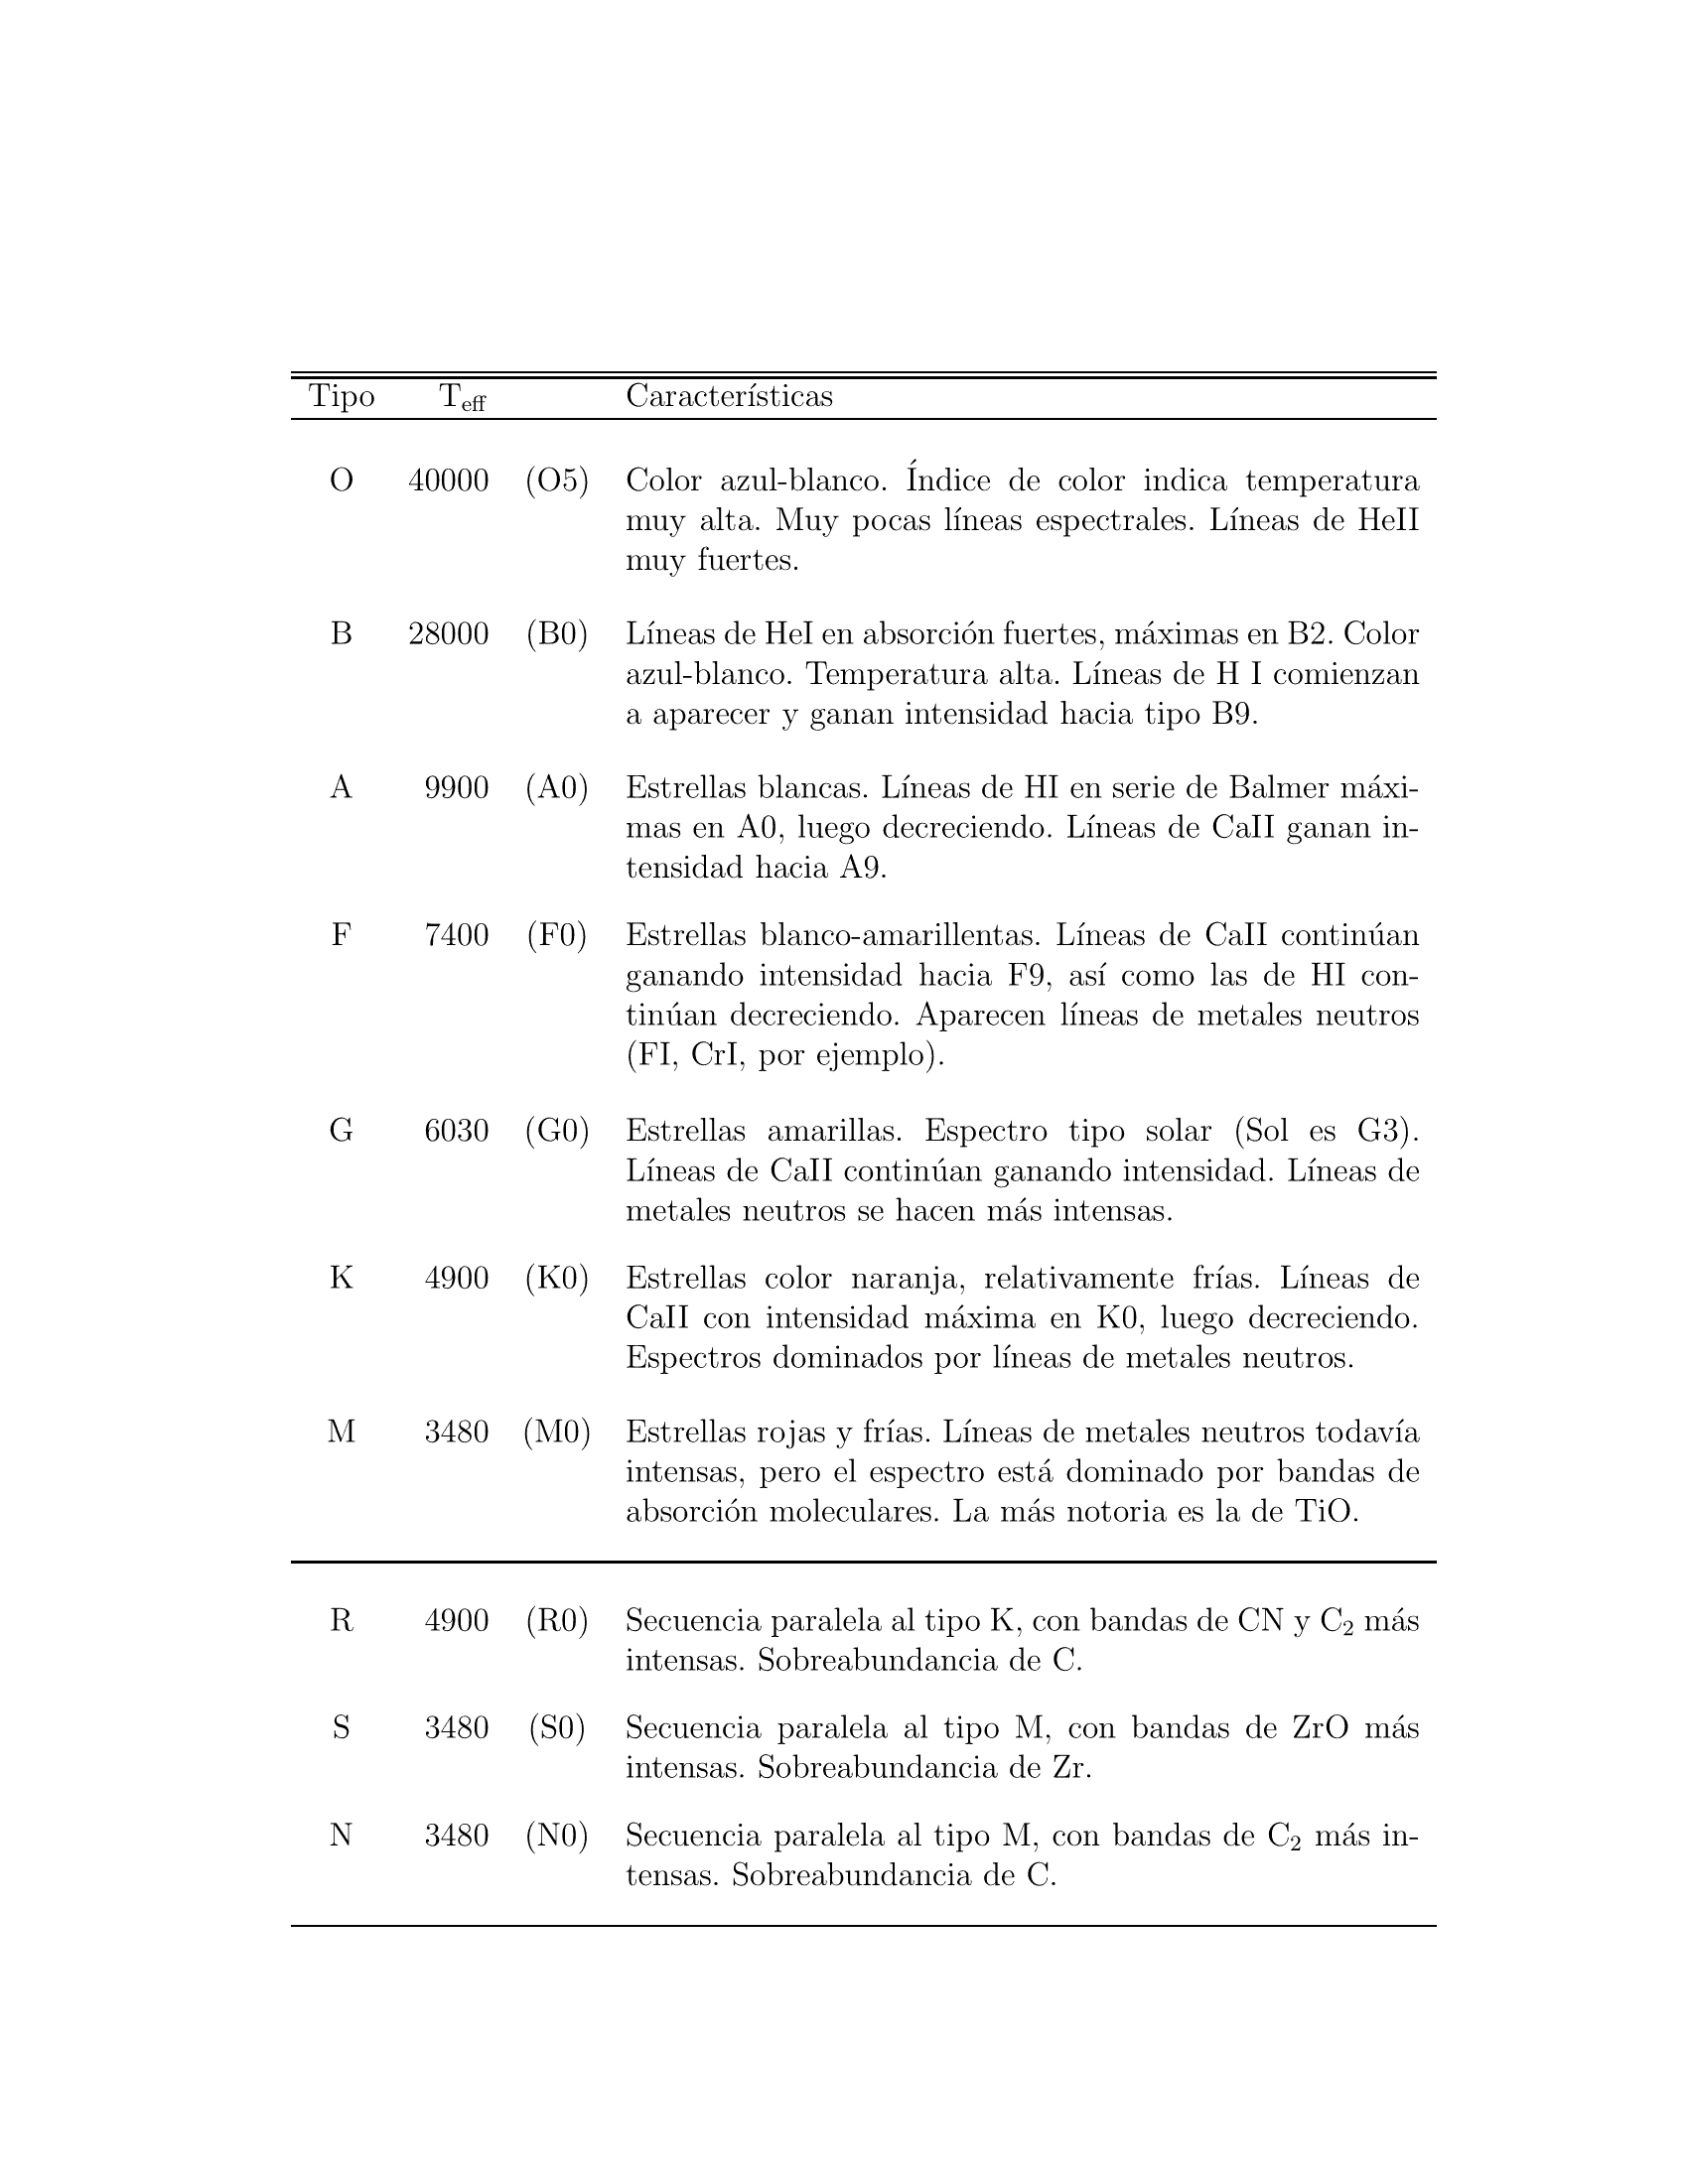
\includegraphics[width=0.98\textwidth]{tabla.png} 
\end{tabular}
\caption{{\small Tabla de algunas caracter'isticas para los distintos tipos espectrales extra'idas del libro ``Radiaci'on y Materia en Astrof'isica'' de Clocchiatti \& Catel'an (Tabla 7.1). En ella se pueden observar las distintas temperaturas (en Kelvin) para los distintos tipos espectrales. All'i tambi'en est'an los tipos R, S y N; clasificaciones que fueron originalmente consideradas por separado, pero en realidad son estrellas similar a las tipo K o M aunque con algunas l'ineas an'omalas/m'as intensas de lo esperado.}}\label{tabla}
\end{center} 
\end{figure}

\begin{figure}
\centering
  \begin{subfigure}{6cm}
    \centering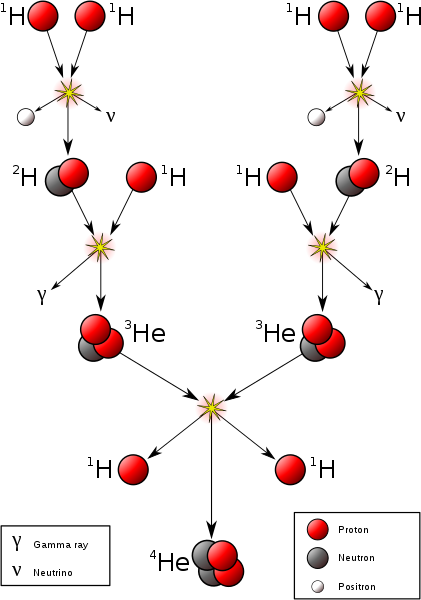
\includegraphics[width=6cm]{p-p.png}
    \caption{Cadena prot'on-prot'on}
  \end{subfigure}
  \begin{subfigure}{6cm}
    \centering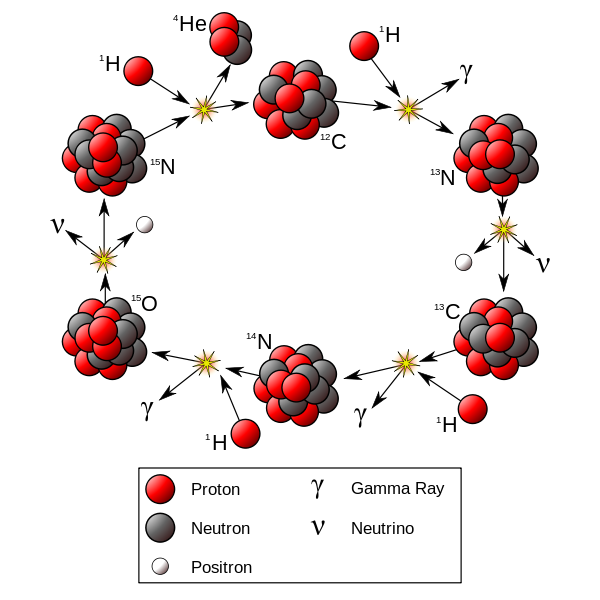
\includegraphics[width=8.5cm]{cno.png}
    \caption{Ciclo CNO}
  \end{subfigure}
  \caption{Distintas reacciones de fusi'on que se pueden generar dentro de una estrella. Cu'al es la que va a dominar depende de la masa de la estrella.}
\end{figure} 
\vspace{3mm}
\end{document}